%Resultados

\section{Resultados}\label{sec:resultados}

    \subsection{Parte 1. Osciladores}\label{subsec:parte1}

        En este apartado se usara la ecuación \ref{eqn:delta_frecuencia}, que nos permite hallar la incertidumbre de las mediciones indirectas de la frecuencias, esta se halla en el apartado \ref{sec:apendice}.
        
        \subsubsection{Sin Control de Amplitud}
            \begin{table}[H]
              \centering
              \begin{tabular}{|c|c|c|c|}
                \hline
                \textbf{Estado} & \textbf{T $[\mu s]$} & \textbf{f [kHz]} & \textbf{$\mathbf{XR_{v1} [\ohm]}$} \\
                \hline
                Inestable & - & - & $0.71(10 \, k) \pm 5 \%$ \\
                \hline
                Inestable & - & - & $0.90(10 \, k) \pm 5 \%$ \\
                \hline
                Inestable & - & - & $0.95(10 \, k) \pm 5 \%$ \\
                \hline
                Oscila & $200 \pm 20$ & $5 \pm 0.5$ & $0.63(10 \, k) \pm 5 \%$ \\
                \hline
                Saturado & $230 \pm 10$ & $4.35 \pm 0.19$ & $0.50(10 \, k) \pm 5 \%$ \\
                \hline
                Saturado & $280 \pm 20$ & $3.57 \pm 0.86$ & $0.40(10 \, k) \pm 5 \%$ \\
                \hline
                Saturado & $600 \pm 40$ & $1.67 \pm 0.11$ & $0.10(10 \, k) \pm 5 \%$ \\
                \hline
              \end{tabular}
              \caption{Mediciones Experimentales de la Figura \ref{fig:puente_wien_control} sin Control de Amplitud}
              \label{tab:exp_puente_wien_sincontrol}
            \end{table}

            Las siguientes imágenes del osciloscopio, corroboran los datos de la tabla \ref{tab:exp_puente_wien_sincontrol}
            
            \begin{figure}[H]
                \centering
                \renewcommand{\figurename}{Imagen}
                \setcounter{figure}{0}
                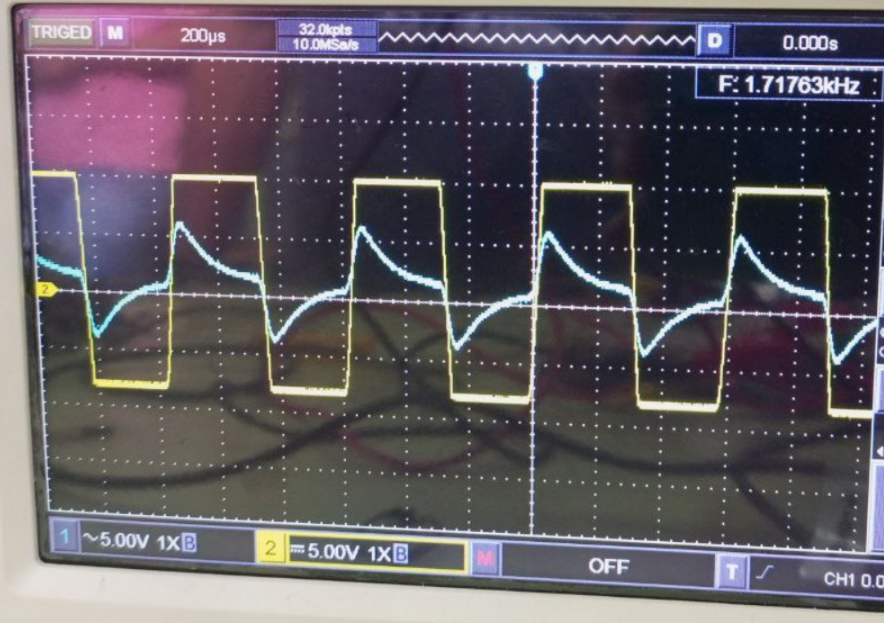
\includegraphics[width=15cm]{Imagenes/exp_puente_wien_sincontrol41.png}
                \caption{Oscilación de la Figura \ref{fig:puente_wien_control} cuando X=0.10}
                \label{fig:exp_puente_wien_sc41}
            \end{figure}

            \begin{table}[H]
                \centering
                \begin{tabular}{|c|c|c|c|}
                    \hline
                    \textbf{time/div} $[s]$ & \textbf{Channel} & \textbf{voltios/div $[\volt]$} & \textbf{Acoplamiento} \\ \hline
                    $(100 \, \pm 20) \mu  $ & 1 (Azul)  &   $5 \pm 1 $ & AC \\ \hline  
                    $(100 \, \pm 20) \mu  $ & 2 (Amarillo)  &   $5 \pm 1 $ & AC \\ \hline  
                \end{tabular}
                \caption{Escalas Usada en el Osciloscopio Digital UNI-T UTD2102CEX+}
                \label{tab:escala_puente_wien_sc41}
            \end{table}
            
            \begin{figure}[H]
                \centering
                \renewcommand{\figurename}{Imagen}
                \setcounter{figure}{0}
                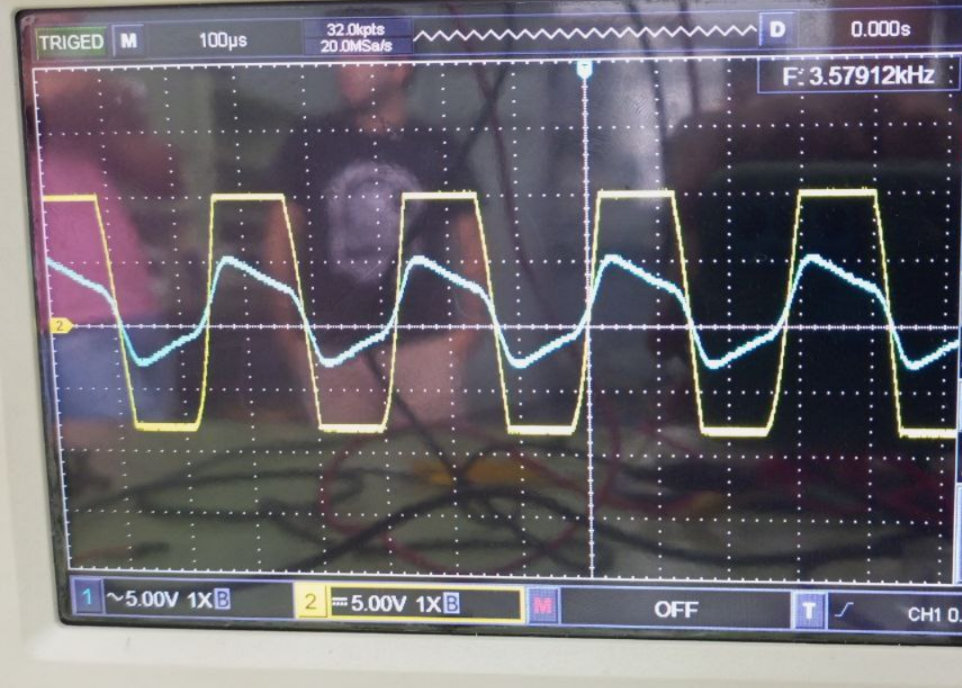
\includegraphics[width=15cm]{Imagenes/exp_puente_wien_sincontrol4.png}
                \caption{Oscilación de la Figura \ref{fig:puente_wien_control} cuando X=0.40}
                \label{fig:exp_puente_wien_sc4}
            \end{figure}

            \begin{table}[H]
                \centering
                \begin{tabular}{|c|c|c|c|}
                    \hline
                    \textbf{time/div} $[s]$ & \textbf{Channel} & \textbf{voltios/div $[\volt]$} & \textbf{Acoplamiento} \\ \hline
                    $(200 \, \pm 40) \mu  $ & 1 (Azul)  &   $5 \pm 1 $ & AC \\ \hline  
                    $(200 \, \pm 40) \mu  $ & 2 (Amarillo)  &   $5 \pm 1 $ & AC \\ \hline  
                \end{tabular}
                \caption{Escalas Usada en el Osciloscopio Digital UNI-T UTD2102CEX+}
                \label{tab:escala_puente_wien_sc4}
            \end{table}

            \begin{figure}[H]
                \centering
                \renewcommand{\figurename}{Imagen}
                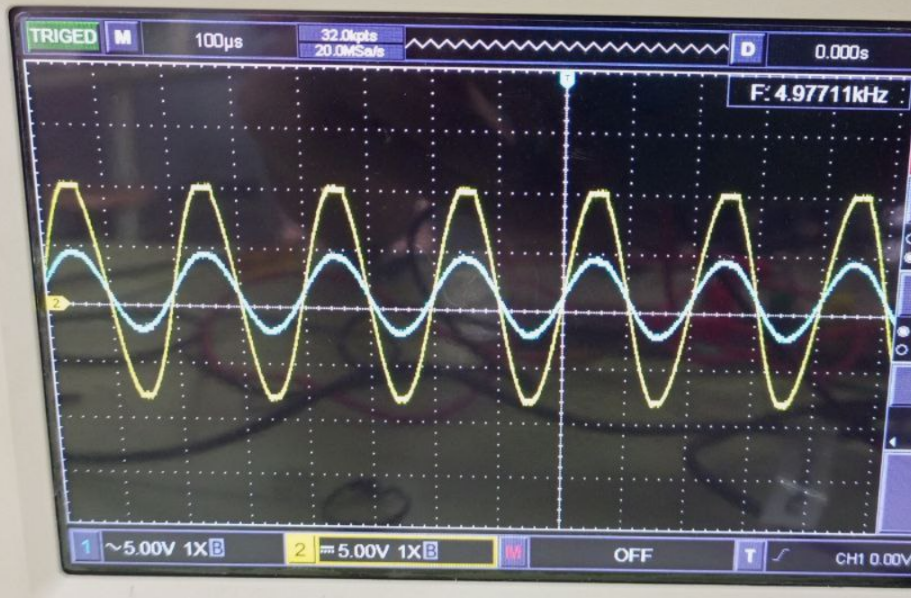
\includegraphics[width=15cm]{Imagenes/exp_puente_wien_sc63.png}
                \caption{Saturación de la Figura \ref{fig:puente_wien_control} cuando X=0.63}
                \label{fig:exp_puente_wien_sc63}
            \end{figure}

            \begin{table}[H]
                \centering
                \begin{tabular}{|c|c|c|c|}
                    \hline
                    \textbf{time/div} $[s]$ & \textbf{Channel} & \textbf{voltios/div $[\volt]$} & \textbf{Acoplamiento} \\ \hline
                    $(100 \, \pm 20) \mu  $ & 1 (Azul)  &   $5 \pm 1 $ & AC \\ \hline  
                    $(100 \, \pm 20) \mu  $ & 2 (Amarillo)  &   $5 \pm 1 $ & AC \\ \hline 
                \end{tabular}
                \caption{Escalas Usada en el Osciloscopio Digital UNI-T UTD2102CEX+}
                \label{tab:escala_puente_wien_sc63}
            \end{table}

            \begin{figure}[H]
                \centering
                \renewcommand{\figurename}{Imagen}
                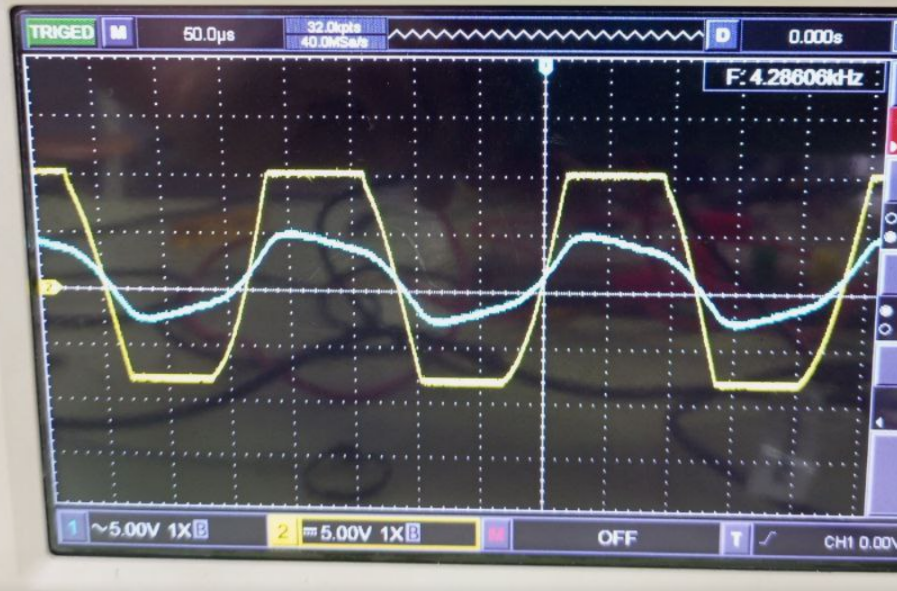
\includegraphics[width=15cm]{Imagenes/exp_puente_wien_sc5.png}
                \caption{Saturación de la Figura \ref{fig:puente_wien_control} cuando X=0.5}
                \label{fig:exp_puente_wien_sc5}
            \end{figure}

            \begin{table}[H]
                \centering
                \begin{tabular}{|c|c|c|c|}
                    \hline
                    \textbf{time/div} $[s]$ & \textbf{Channel} & \textbf{voltios/div $[\volt]$} & \textbf{Acoplamiento} \\ \hline
                    $(50 \, \pm 10) \mu  $ & 1 (Azul)  &   $5 \pm 1 $ & AC \\ \hline  
                    $(50 \, \pm 10) \mu  $ & 2 (Amarillo)  &   $5 \pm 1 $ & AC \\ \hline 
                \end{tabular}
                \caption{Escalas Usada en el Osciloscopio Digital UNI-T UTD2102CEX+}
                \label{tab:escala_puente_wien_sc5}
            \end{table}

            \begin{figure}[H]
                \centering
                \renewcommand{\figurename}{Imagen}
                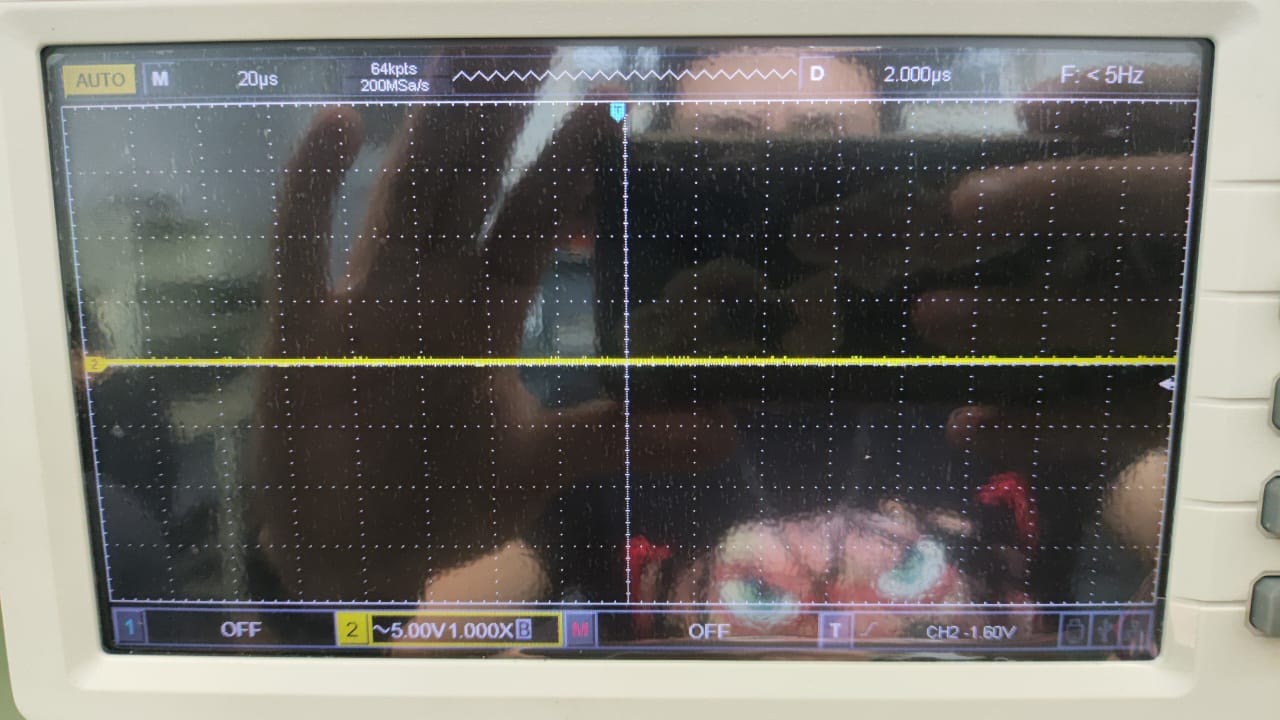
\includegraphics[width=15cm]{Imagenes/exp_puente_wien_sc9.jpg}
                \caption{Punto critico del Estado en Corte de la Figura \ref{fig:puente_wien_control} cuando X=0.95}
                \label{fig:exp_puente_wien_sc9}
            \end{figure}

            \begin{table}[H]
                \centering
                \begin{tabular}{|c|c|c|c|}
                    \hline
                    \textbf{time/div} $[s]$ & \textbf{Channel} & \textbf{voltios/div $[\volt]$} & \textbf{Acoplamiento} \\ \hline
                    $(20 \, \pm 4) \mu  $ & 2 (Amarillo)  &   $5 \pm 1 $ & AC \\ \hline  
                \end{tabular}
                \caption{Escalas Usada en el Osciloscopio Digital UNI-T UTD2102CEX+}
                \label{tab:escala_puente_wien_sc9}
            \end{table}


            Si se observan las tablas \ref{tab:sim_puente_wien_sc} y \ref{tab:exp_puente_wien_sincontrol}, se pueden obtener sus desviaciones estándar para evidenciar que el diseño realizado fueron los adecuados.

            \begin{table}[H]
              \centering
              \begin{tabular}{|c|c|c|c|}
                \hline
                $\mathbf{XR_{v1} [\ohm]}$ & $\mathbf{T_{Teorico} [\mu s]}$ & $\mathbf{T_{Experimenta}[\mu s]}$ & $\mathbf{Desv [\%]}$ \\
                \hline
                $0.60(10 \, k)$ & - & - & 0 \\
                \hline
                $0.598(10 \, k)$ & $213.4$ & $200 \pm 40$ & 6.28 \\
                \hline
                $0.50(10 \, k)$ & $240.38$ & $230 \pm 10$ & 4.32 \\
                \hline
                $0.10(10 \, k)$ & $540.54$ & $600 \pm 40$ & 11 \\
                \hline
              \end{tabular}
              \caption{Desviación estándar del periodo de la Figura \ref{fig:puente_wien_control} sin control de amplitud.}
              \label{tab:desviacion_puente_wien_sc}
            \end{table}
            


        \subsubsection{Con Control de Amplitud}

            \begin{table}[H]
              \centering
              \begin{tabular}{|c|c|c|c|}
                \hline
                \textbf{Estado} & $\mathbf{T [\mu s]}$ & \textbf{f [kHz]} & $\mathbf{XR_{v1} [\ohm]}$ \\
                \hline
                Corte & - & - & $0.90(10 \, k) \pm 5 \%$ \\
                \hline
                Oscilación & $200 \pm 20$ & $5.00 \pm 0.50$ & $0.40(10 \, k) \pm 5 \%$ \\
                \hline
                Saturación & $520 \pm 40$ & $1.92 \pm 0.14$ & $0.10(10 \, k) \pm 5 \%$ \\
                \hline
              \end{tabular}
              \caption{Mediciones Experimentales de la Figura \ref{fig:puente_wien_control} con Control de Amplitud}
              \label{tab:exp_puente_wien_control}
            \end{table}

            De igual manera, que con las mediciones experimentales del Puente de Wien sin control de amplitud, en las siguientes imágenes del osciloscopio, corroboran los datos de la tabla \ref{tab:exp_puente_wien_control} 
            
            \begin{figure}[H]
                \centering
                \renewcommand{\figurename}{Imagen}
                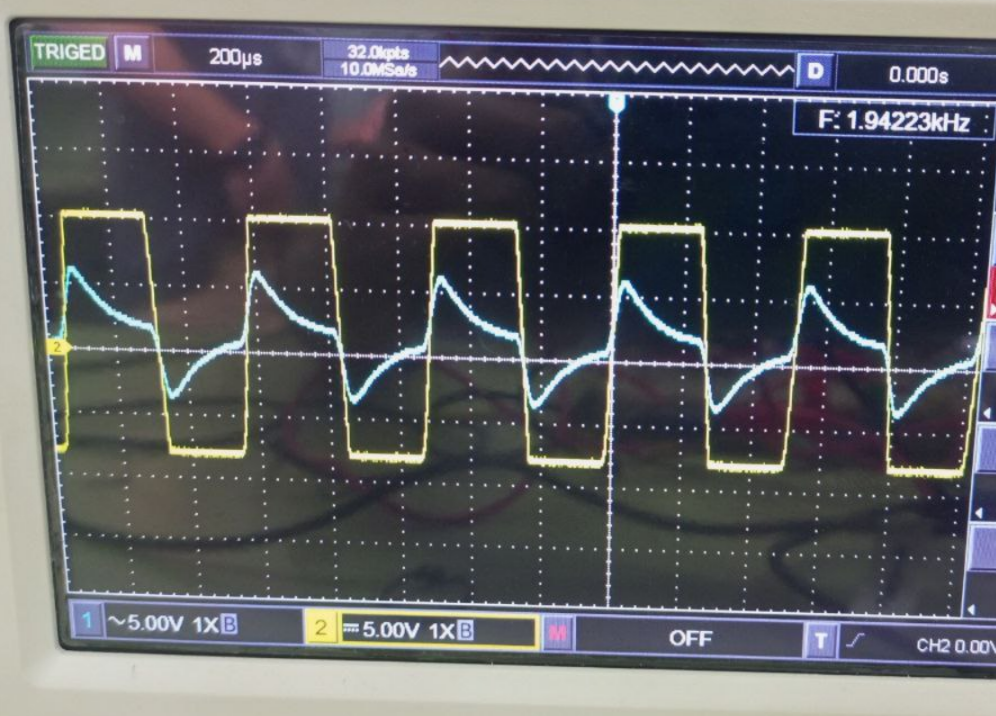
\includegraphics[width=15cm]{Imagenes/exp_puente_wien_control0.png}
                \caption{Estado de Saturación con el control de amplitud de la Figura \ref{fig:puente_wien_control} cuando X=0.1}
                \label{fig:exp_puente_wien_control0}
            \end{figure}

            \begin{table}[H]
                \centering
                \begin{tabular}{|c|c|c|c|}
                    \hline
                    \textbf{time/div} $[s]$ & \textbf{Channel} & \textbf{voltios/div $[\volt]$} & \textbf{Acoplamiento} \\ \hline
                    $(200 \, \pm 40) \mu  $ & 1 (Azul)  &   $5 \pm 1 $ & AC \\ \hline  
                    $(200 \, \pm 40) \mu  $ & 2 (Amarillo)  &   $5 \pm 1 $ & AC \\ \hline   
                \end{tabular}
                \caption{Escalas Usada en el Osciloscopio Digital UNI-T UTD2102CEX+}
                \label{tab:escala_puente_wien_control0}
            \end{table}
            
            \begin{figure}[H]
                \centering
                \renewcommand{\figurename}{Imagen}
                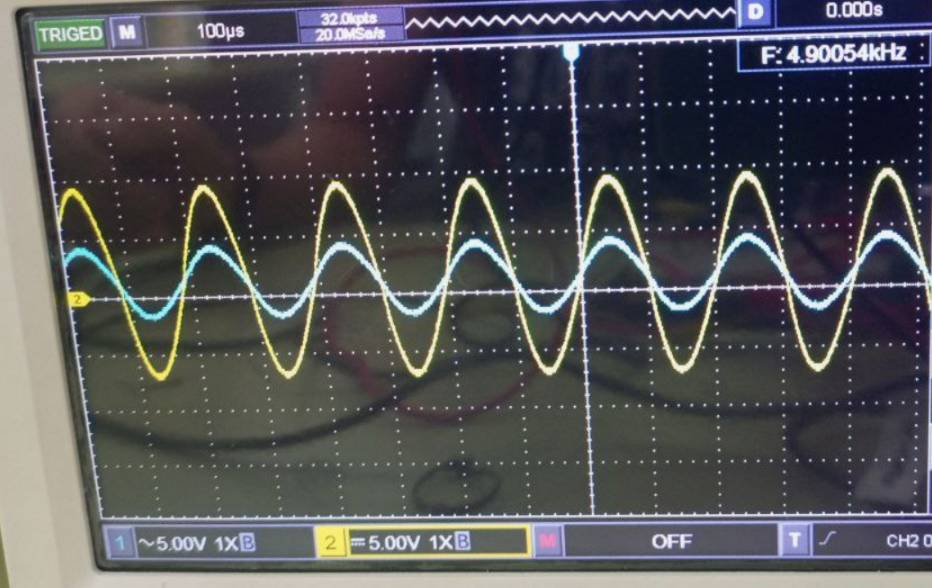
\includegraphics[width=15cm]{Imagenes/exp_puente_wien_control45.png}
                \caption{Estado de Oscilación con el control de amplitud de la Figura \ref{fig:puente_wien_control} cuando X=0.4}
                \label{fig:exp_puente_wien_control45}
            \end{figure}

            \begin{table}[H]
                \centering
                \begin{tabular}{|c|c|c|c|}
                    \hline
                    \textbf{time/div} $[s]$ & \textbf{Channel} & \textbf{voltios/div $[\volt]$} & \textbf{Acoplamiento} \\ \hline
                    $(100 \, \pm 20) \mu  $ & 1 (Azul)  &   $(5 \pm 1)  \, m $ & AC \\ \hline  
                    $(100 \, \pm 20) \mu  $ & 2 (Amarillo)  &   $(5 \pm 1)  \, m $ & AC \\ \hline  
                \end{tabular}
                \caption{Escalas Usada en el Osciloscopio Digital UNI-T UTD2102CEX+}
                \label{tab:escala_puente_wien_control45}
            \end{table}

            
            \begin{figure}[H]
                \centering
                \renewcommand{\figurename}{Imagen}
                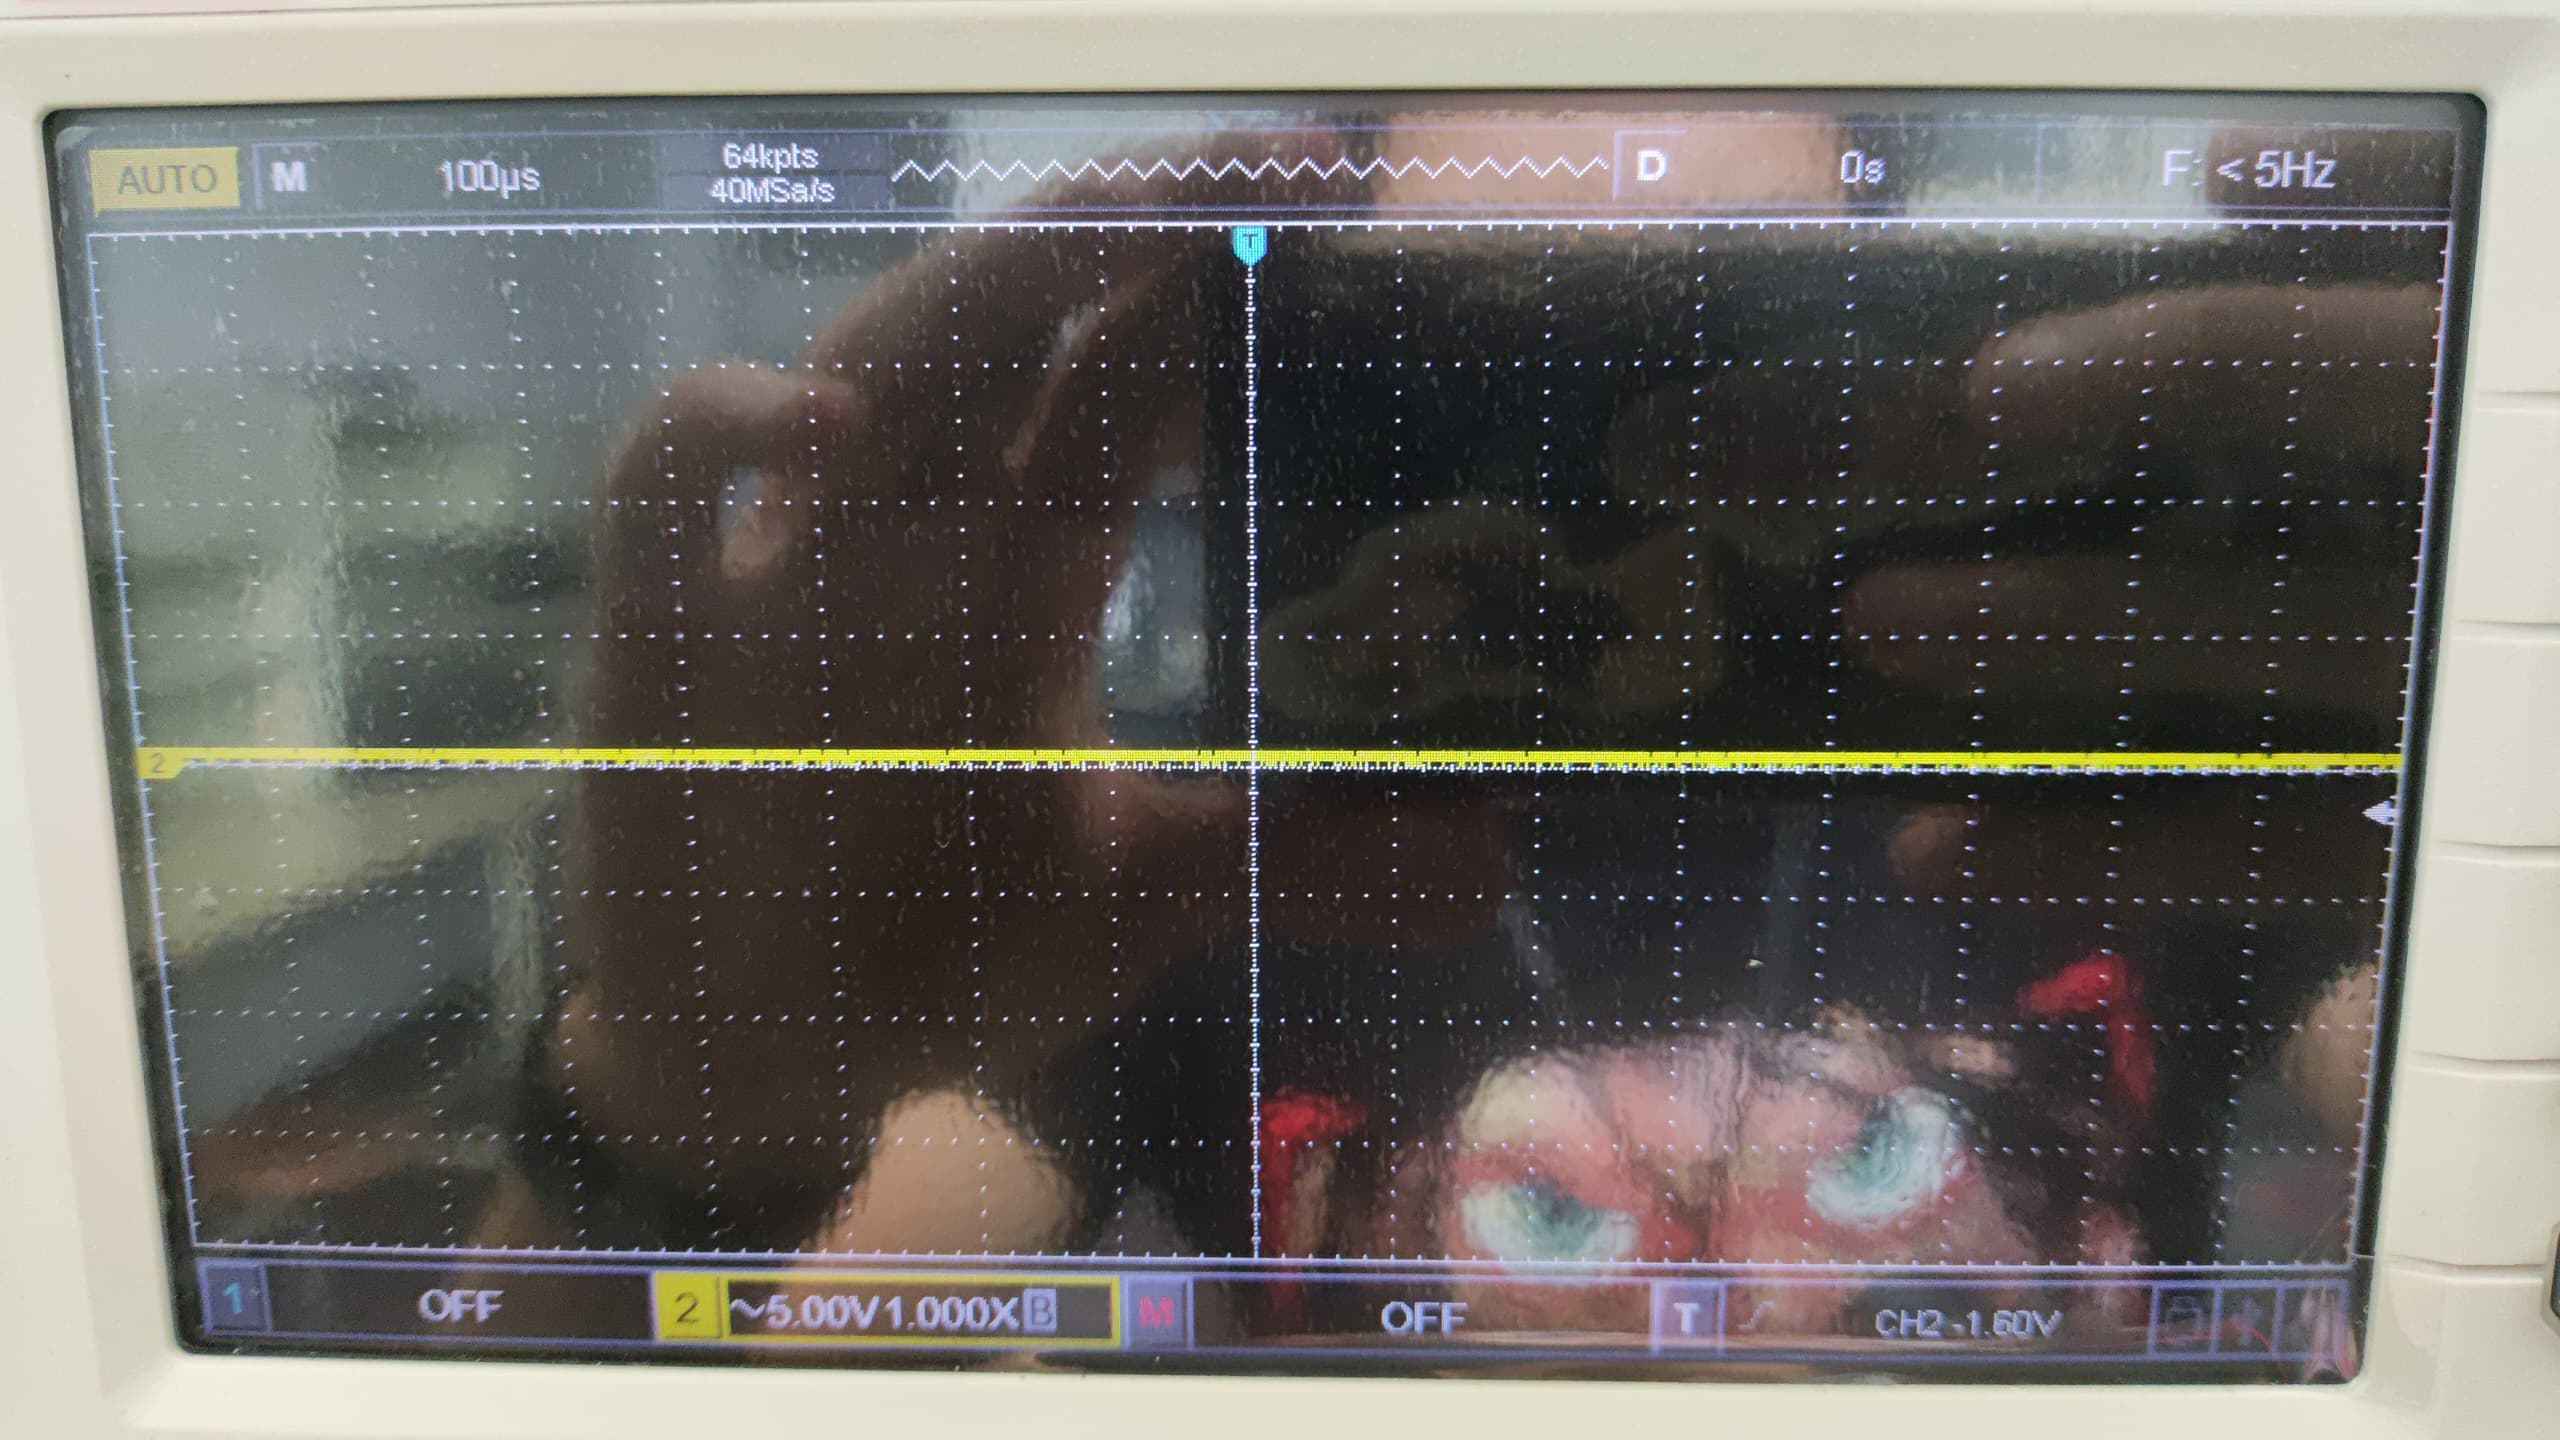
\includegraphics[width=15cm]{Imagenes/exp_puente_wien_control9.jpg}
                \caption{Estado de Corte con el control de amplitud de la Figura \ref{fig:puente_wien_control} cuando X=0.9}
                \label{fig:exp_puente_wien_control9}
            \end{figure}

            \begin{table}[H]
                \centering
                \begin{tabular}{|c|c|c|c|}
                    \hline
                    \textbf{time/div} $[s]$ & \textbf{Channel} & \textbf{voltios/div $[\volt]$} & \textbf{Acoplamiento} \\ \hline
                    $(100 \, \pm 20) \mu  $ & 2 (Amarillo)  &   $5 \pm 1 $ & AC \\ \hline  
                \end{tabular}
                \caption{Escalas Usada en el Osciloscopio Digital UNI-T UTD2102CEX+}
                \label{tab:escala_puente_wien_control9}
            \end{table}

             Si se observan las tablas \ref{tab:sim_puente_wien_control} y \ref{tab:exp_puente_wien_control}, se pueden obtener sus desviaciones estándar para evidenciar que el diseño realizado fueron los adecuados.
             
             \begin{table}[H]
                 \centering
                  \begin{tabular}{|c|c|c|c|}
                    \hline
                    $\mathbf{XR_{v1} [\ohm]}$ & $\mathbf{T_{Teorico} [\mu s]}$ & $\mathbf{T_{Experimental}[\mu s]}$ & $\mathbf{Desv [\%]}$ \\
                    \hline
                    $0.90 \, (10 \, k)$ & - & - & 0 \\
                    \hline
                    $0.40 \, (10 \, k)$ & $223.26$ & $200 \pm 20$ & 10.42 \\
                    \hline
                    $0.10 \, (10 \, k)$ & $314.46$ & $520 \pm 80$ & 65.36 \\
                    \hline
                  \end{tabular}
                  \caption{Desviación estándar del periodo de la Figura \ref{fig:puente_wien_control} con control de amplitud.}
                  \label{tab:desviacion_puente_wien_control}
                \end{table}


    \subsection{Parte 2. Multivibradores}\label{subsec:parte2}

        En este apartado se mostraran los resultado medidos en el laboratorio de la sección \ref{sec:metodologia} en su subsección \ref{subsec:meto_parte2}, obteniendo los siguiente:
        
        \subsubsection{Multivibrador Astable}

            \begin{table}[H]
              \centering
              \begin{tabular}{|c|c|c|c|}
                \hline
                $\mathbf{V_c [V_p]}$ & $\mathbf{V_p ^+[V_p]}$ & $\mathbf{f [KHz]}$ & $\mathbf{T [\mu s]}$ \\
                \hline
                $3 \pm 0.2$ & $2.8 \pm 0.2$ & $4.55 \pm 0.21$ & $220 \pm 10$ \\
                \hline
              \end{tabular}
              \caption{Mediciones experimentales del circuito \ref{fig:astable}.}
              \label{tab:exp_astable}
            \end{table}

            Al realizar su debidos cálculos de error para verificar si los datos del diseño fueron los adecuados para el laboratorio.

            \begin{table}[H]
              \centering
              \begin{tabular}{|c|c|c|c|c|c|}
                \hline
                $\mathbf{V_{CTeorico} [\mu s]}$ & $\mathbf{V_{CExperimental}[\mu s]}$ & $\mathbf{Desv [\%]}$ & $\mathbf{f_{Teorico} [\mu s]}$ & $\mathbf{f_{Experimental}[\mu s]}$ & $\mathbf{Desv [\%]}$ \\
                \hline
                $2$ & $3 \pm 0.2$ & $50$ & $5$ & $4.55 \pm 0.21$ & $9$ \\
                \hline
              \end{tabular}
              \caption{Desviación estándar de las mediciones de la tabla \ref{tab:exp_astable}.}
              \label{tab:desv_astable}
            \end{table}

            \begin{figure}[H]
                \centering
                \renewcommand{\figurename}{Imagen}
                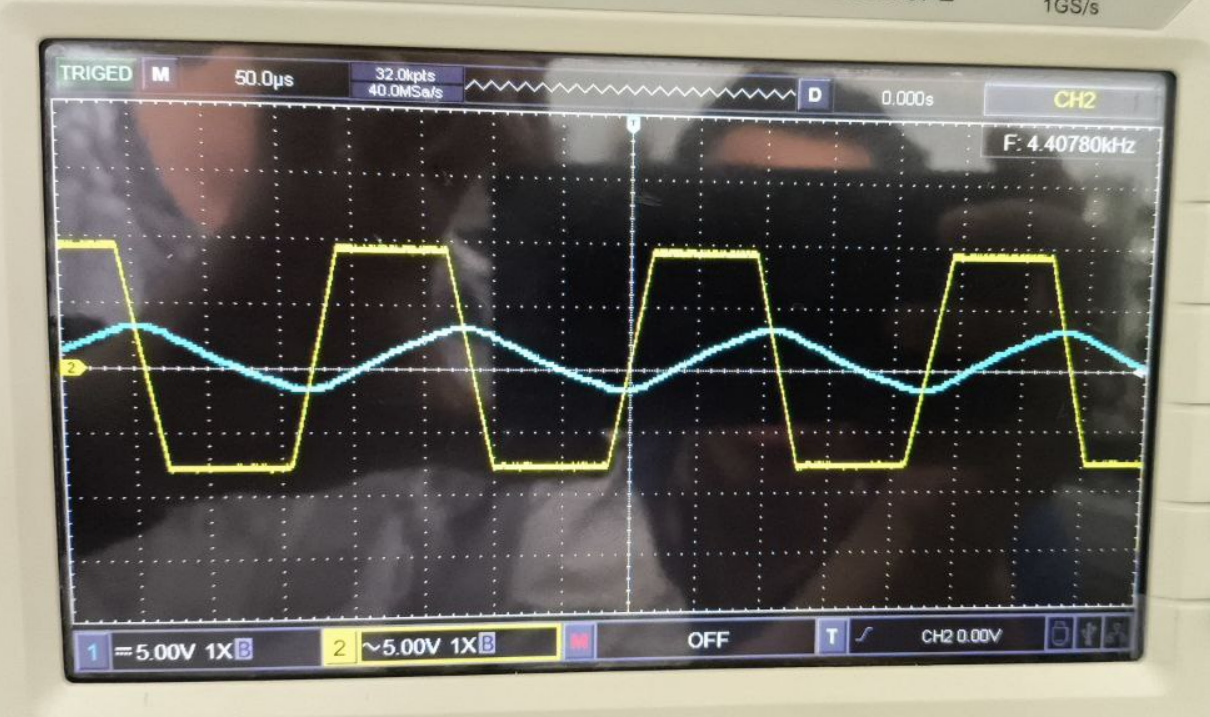
\includegraphics[width=15cm]{Imagenes/exp_astable_vc_vout.png}
                \caption{Señales de salida de la figura \ref{fig:astable}. Vout:salida del circuito \ref{fig:astable} (Amarillo), Vc:Salida del capacitor (Azul)}
                \label{fig:exp_astable_vc_vout}
            \end{figure}

            \begin{table}[H]
                \centering
                \begin{tabular}{|c|c|c|c|}
                    \hline
                    \textbf{time/div} $[s]$ & \textbf{Channel} & \textbf{voltios/div $[\volt]$} & \textbf{Acoplamiento} \\ \hline
                    $(50 \, \pm 10) \mu  $ & 1 (Azul)  &   $5 \pm 1   $ & AC \\ \hline  
                    $(50 \, \pm 10) \mu  $ & 2 (Amarillo)  &   $5 \pm 1   $ & AC \\ \hline  
                \end{tabular}
                \caption{Escalas Usada en el Osciloscopio Digital UNI-T UTD2102CEX+}
                \label{tab:escala_astable_vc_vout}
            \end{table}

            \begin{figure}[H]
                \centering
                \renewcommand{\figurename}{Imagen}
                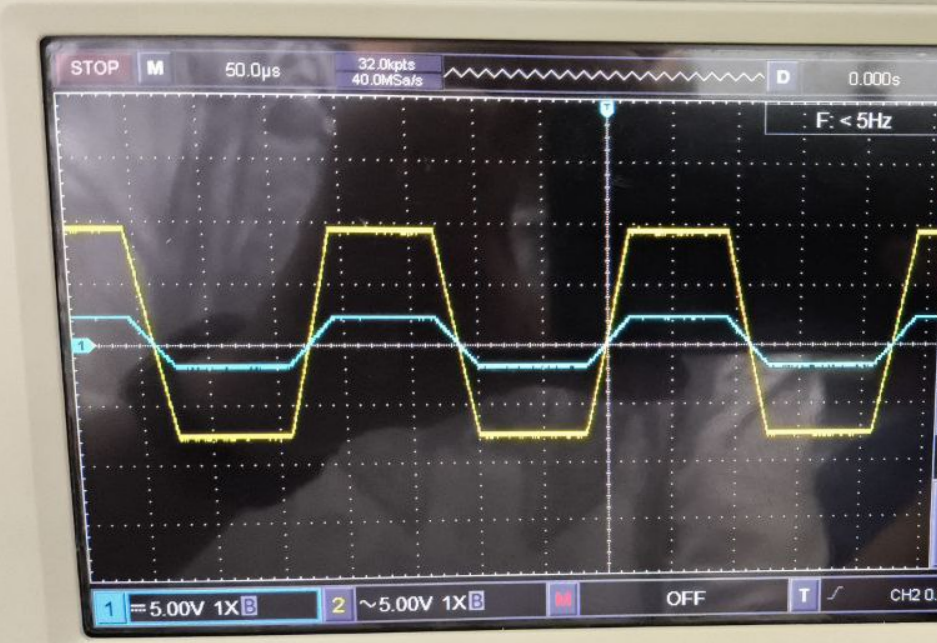
\includegraphics[width=15cm]{Imagenes/exp_astable_vp_vout.png}
                \caption{Señales de salida de la figura \ref{fig:astable}. Vout:salida del circuito \ref{fig:astable} (Amarillo), Vp:Salida de la entrada no inversora (Azul)}
                \label{fig:exp_astable_vp_vout}
            \end{figure}

            \begin{table}[H]
                \centering
                \begin{tabular}{|c|c|c|c|}
                    \hline
                    \textbf{time/div} $[s]$ & \textbf{Channel} & \textbf{voltios/div $[\volt]$} & \textbf{Acoplamiento} \\ \hline
                    $(50 \, \pm 10) \mu  $ & 1 (Azul)  &   $5 \pm 1   $ & AC \\ \hline  
                    $(50 \, \pm 10) \mu  $ & 2 (Amarillo)  &   $5 \pm 1   $ & AC \\ \hline  
                \end{tabular}
                \caption{Escalas Usada en el Osciloscopio Digital UNI-T UTD2102CEX+}
                \label{tab:escala_astable_vp_vout}
            \end{table}


        \subsubsection{Multivibrador Monoestable}

            \begin{table}[H]
              \centering
              \begin{tabular}{|c|c|c|c|c|c|c|}
                \hline
                $\mathbf{V_{out} [V_{pp}]}$ & $\mathbf{V_D [V_{DC}]}$ & $\mathbf{V_{pulso} [V_{DC}]}$ & $\mathbf{V_c [V_{pp}]}$ & $\mathbf{T_{pulso} [ms]}$ & $\mathbf{f_{pulso} [Hz]}$ & $\mathbf{f_{max} [Hz]}$ \\
                \hline
                $17 \pm 1$ & $1.2 \pm 0.2$ & $-5 \pm 1$ & $3.2 \pm 0.4$ & $4 \pm 0.4$ & $250 \pm 25$ & $41 \pm 1.68$ \\
                \hline
              \end{tabular}
              \caption{Mediciones Experimentales del Circuito \ref{fig:monoestable}. Características importantes del circuito.}
              \label{tab:exp_monoestable}
            \end{table}

            

            
            \begin{figure}[H]
                \centering
                \renewcommand{\figurename}{Imagen}
                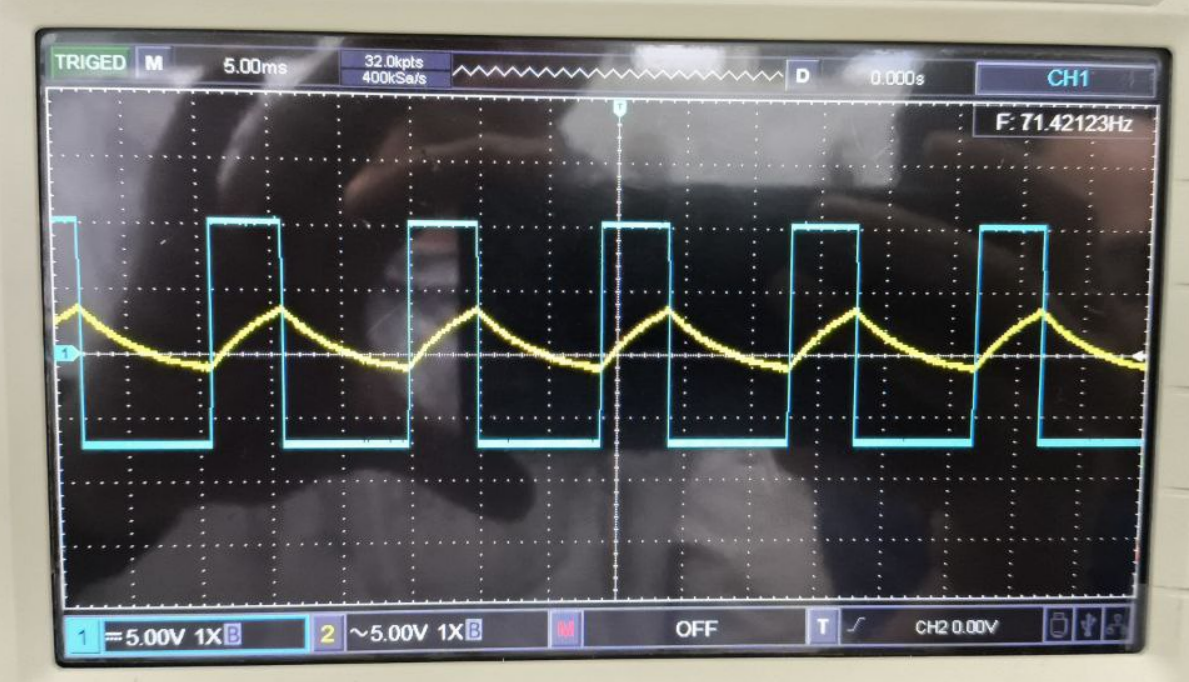
\includegraphics[width=15cm]{Imagenes/exp_monoestable_vc_vout.png}
                \caption{Señales de salida de la figura \ref{fig:monoestable}. Vout:salida del circuito (Azul), Vc6=VD:Voltaje del capacitor en paralelo con el LED (Amarillo)}
                \label{fig:exp_monoestable_vc_vout}
            \end{figure}

            \begin{table}[H]
                \centering
                \begin{tabular}{|c|c|c|c|}
                    \hline
                    \textbf{time/div} $[s]$ & \textbf{Channel} & \textbf{voltios/div $[\volt]$} & \textbf{Acoplamiento} \\ \hline
                    $(5 \, \pm 2) \, m  $ & 1 (Azul)  &   $5 \pm 1   $ & AC \\ \hline  
                    $(5 \, \pm 2) \, m  $ & 2 (Amarillo)  &   $5 \pm 1   $ & AC \\ \hline  
                \end{tabular}
                \caption{Escalas Usada en el Osciloscopio Digital UNI-T UTD2102CEX+}
                \label{tab:escala_monoestable_vc_vout}
            \end{table}

            

            
            \begin{figure}[H]
                \centering
                \renewcommand{\figurename}{Imagen}
                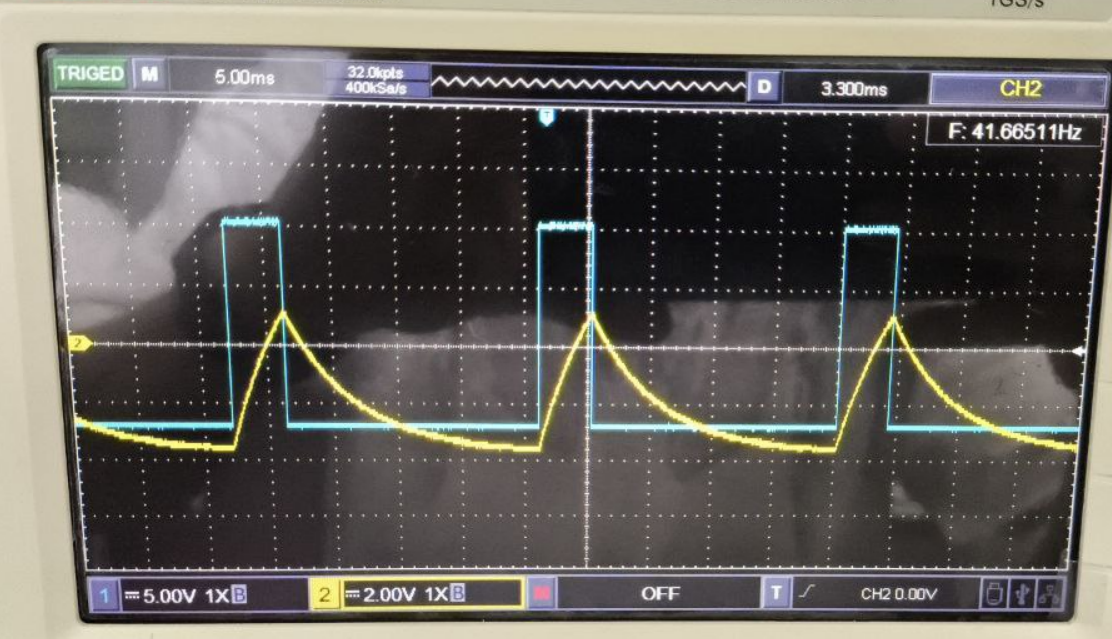
\includegraphics[width=15cm]{Imagenes/exp_monoestable_vc_vout_dc.png}
                \caption{Señales de salida de la figura \ref{fig:monoestable}. Vout:salida del circuito (Azul), Vc6=VD:Voltaje del capacitor en paralelo con el LED (Amarillo)}
                \label{fig:exp_monoestable_vc_vout_dc}
            \end{figure}

            \begin{table}[H]
                \centering
                \begin{tabular}{|c|c|c|c|}
                    \hline
                    \textbf{time/div} $[s]$ & \textbf{Channel} & \textbf{voltios/div $[\volt]$} & \textbf{Acoplamiento} \\ \hline
                    $(5 \, \pm 2) \, m  $ & 1 (Azul)  &   $5 \pm 1   $ & DC \\ \hline  
                    $(5 \, \pm 2) \, m  $ & 2 (Amarillo)  &   $5 \pm 1   $ & DC \\ \hline  
                \end{tabular}
                \caption{Escalas Usada en el Osciloscopio Digital UNI-T UTD2102CEX+}
                \label{tab:escala_monoestable_vc_vout_dc}
            \end{table}

            
            \begin{figure}[H]
                \centering
                \renewcommand{\figurename}{Imagen}
                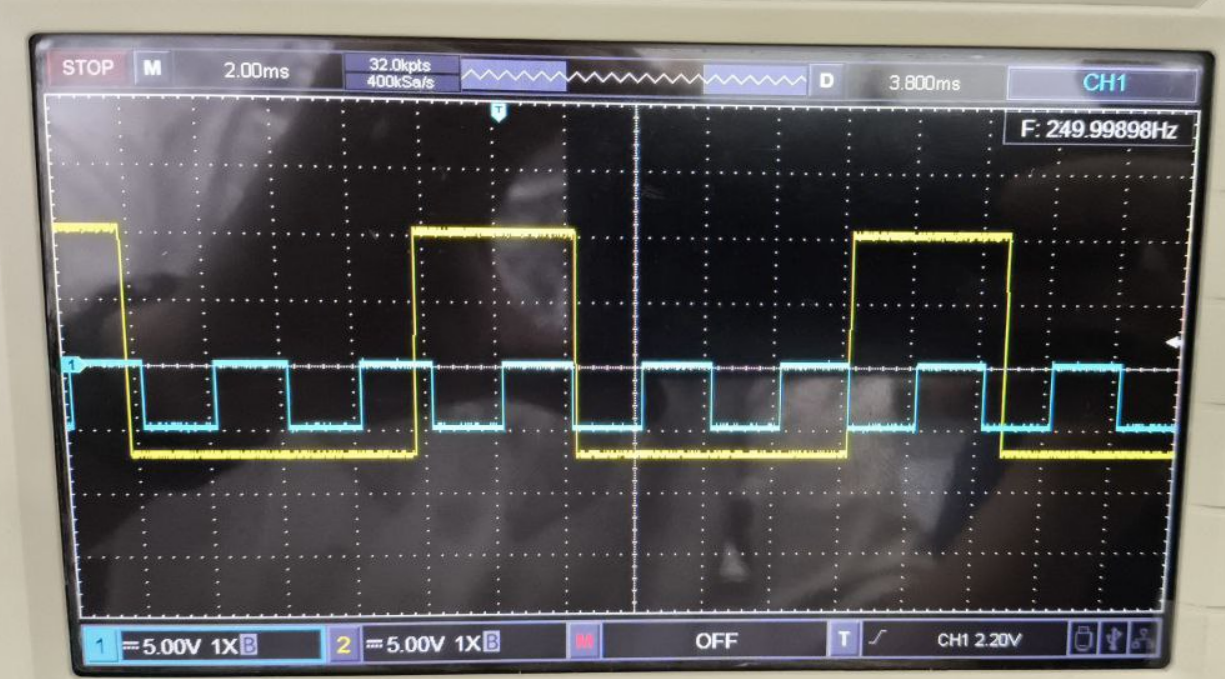
\includegraphics[width=15cm]{Imagenes/exp_monoestable_vin_vout.png}
                \caption{Señales de salida de la figura \ref{fig:monoestable}. Vout:salida del circuito (Amarillo), Vin:Salida del generador de funciones (Azul)}
                \label{fig:exp_monoestable_vin_vout}
            \end{figure}

            \begin{table}[H]
                \centering
                \begin{tabular}{|c|c|c|c|}
                    \hline
                    \textbf{time/div} $[s]$ & \textbf{Channel} & \textbf{voltios/div $[\volt]$} & \textbf{Acoplamiento} \\ \hline
                    $(2 \, \pm 0.4) \, m  $ & 1 (Azul)  &   $5 \pm 1   $ & AC \\ \hline  
                    $(2 \, \pm 0.4) \, m  $ & 2 (Amarillo)  &   $5 \pm 1   $ & AC \\ \hline  
                \end{tabular}
                \caption{Escalas Usada en el Osciloscopio Digital UNI-T UTD2102CEX+}
                \label{tab:escala_monoestable_vin_vout}
            \end{table}

            
            \begin{figure}[H]
                \centering
                \renewcommand{\figurename}{Imagen}
                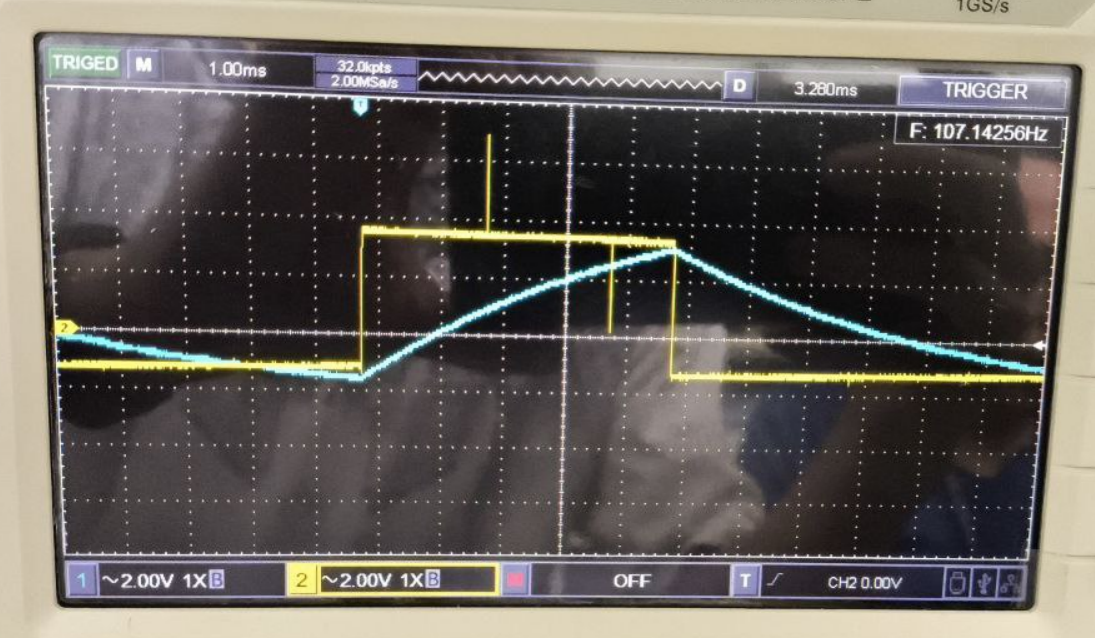
\includegraphics[width=15cm]{Imagenes/exp_monoestable_vd_vcmage 2024-02-08 at 11.29.33_3958794e.png}
                \caption{Señales de salida de la figura \ref{fig:monoestable}. VD:salida de la entrada no inversora o catodo del diodo (Amarillo), Vc6:Voltaje de capacitor 6 en paralelo con el LED (Azul).}
                \label{fig:exp_monoestable_vcat_vc}
            \end{figure}

            \begin{table}[H]
                \centering
                \begin{tabular}{|c|c|c|c|}
                    \hline
                    \textbf{time/div} $[s]$ & \textbf{Channel} & \textbf{voltios/div $[\volt]$} & \textbf{Acoplamiento} \\ \hline
                    $(1 \, \pm 0.2) \, m  $ & 1 (Azul)  &   $2 \pm 0.4   $ & AC \\ \hline  
                    $(1 \, \pm 0.2) \, m  $ & 2 (Amarillo)  &   $2 \pm 0.4   $ & AC \\ \hline  
                \end{tabular}
                \caption{Escalas Usada en el Osciloscopio Digital UNI-T UTD2102CEX+}
                \label{tab:escala_monoestable_vcat_vc}
            \end{table}

            
            \begin{figure}[H]
                \centering
                \renewcommand{\figurename}{Imagen}
                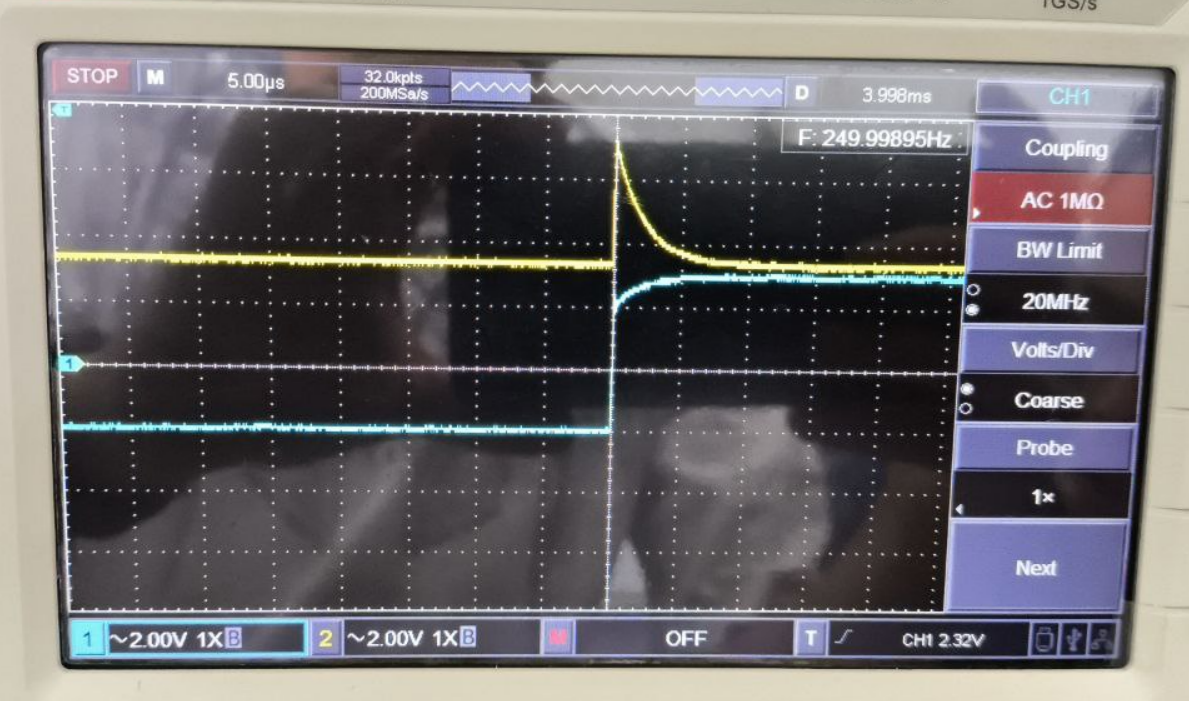
\includegraphics[width=15cm]{Imagenes/exp_monoestable_vcat_vin.png}
                \caption{Señales de salida de la figura \ref{fig:monoestable}. Ciclo de carga y descarga del capacitor,  VD:salida de la entrada no inversora o cátodo del diodo (Amarillo), Vin:Voltaje de entrada del pulso negativo (Azul)}
                \label{fig:exp_monoestable_vcat_vin}
            \end{figure}

            \begin{table}[H]
                \centering
                \begin{tabular}{|c|c|c|c|}
                    \hline
                    \textbf{time/div} $[s]$ & \textbf{Channel} & \textbf{voltios/div $[\volt]$} & \textbf{Acoplamiento} \\ \hline
                    $(5 \, \pm 1) \, \mu  $ & 1 (Azul)  &   $2 \pm 0.4   $ & AC \\ \hline  
                    $(5 \, \pm 1) \, \mu  $ & 2 (Amarillo)  &   $2 \pm 0.4   $ & AC \\ \hline  
                \end{tabular}
                \caption{Escalas Usada en el Osciloscopio Digital UNI-T UTD2102CEX+}
                \label{tab:escala_monoestable_vcat_vin}
            \end{table}

            

            
            
    
    \subsection{Parte 3. Generador de Funciones}\label{subsec:parte3}

        En este apartado daremos resultados de las mediciones realizada en el laboratorio, del apartado \ref{sec:metodologia} de la sección \ref{subsec:met_parte3}.

        \begin{table}[H]
          \centering
          \begin{tabular}{|c|c|c|c|c|c|}
            \hline
            $\mathbf{V_{out} [V_{pp}]}$ & $\mathbf{V_a [V_{pp}]}$ & $\mathbf{V^+ [V_{pp}]}$ & $\mathbf{T [\mu s]}$ & $\mathbf{f [KHz]}$ & $\mathbf{V_z [V]}$ \\
            \hline
            $17 \pm 1$ & $3.7 \pm 0.1$ & $4.6 \pm 0.4$ & $280 \pm 20$ & $3.57 \pm 0.254$ & $5.1$ \\
            \hline
          \end{tabular}
          \caption{Mediciones experimentales del circuito \ref{fig:gf}.}
          \label{tab:exp_gf}
        \end{table}




        \begin{table}[H]
          \centering
          \begin{tabular}{|c|c|c|c|}
            \hline
            & $\mathbf{Teorico}$ & $\mathbf{Experimental}$ & $\mathbf{Desv [\%]}$ \\
            \hline
            $\mathbf{V_{out} [V_p]}$ & $6$ & $8.5 \pm 1$ & $41.6$ \\
            \hline
            $\mathbf{V_a [V_p]}$ & $4.6$ & $1.85 \pm 0.1$ & $59.78$ \\
            \hline
            $\mathbf{V^+ [V_p]}$ & $4.1$ & $2.3 \pm 0.4$ & $43.90$ \\
            \hline
            $\mathbf{T [\mu s]}$ & $200$ & $280 \pm 20$ & $40$ \\
            \hline
            $\mathbf{f [KHz]}$ & $5$ & $3.57$ & $28.6$ \\
            \hline
          \end{tabular}
          \caption{Desviaciones estándar de cada una de las mediciones experimentales de la figura \ref{fig:gf}.}
          \label{tab:desviacion_gf}
        \end{table}

        
         
            \begin{figure}[H]
                \centering
                \renewcommand{\figurename}{Imagen}
                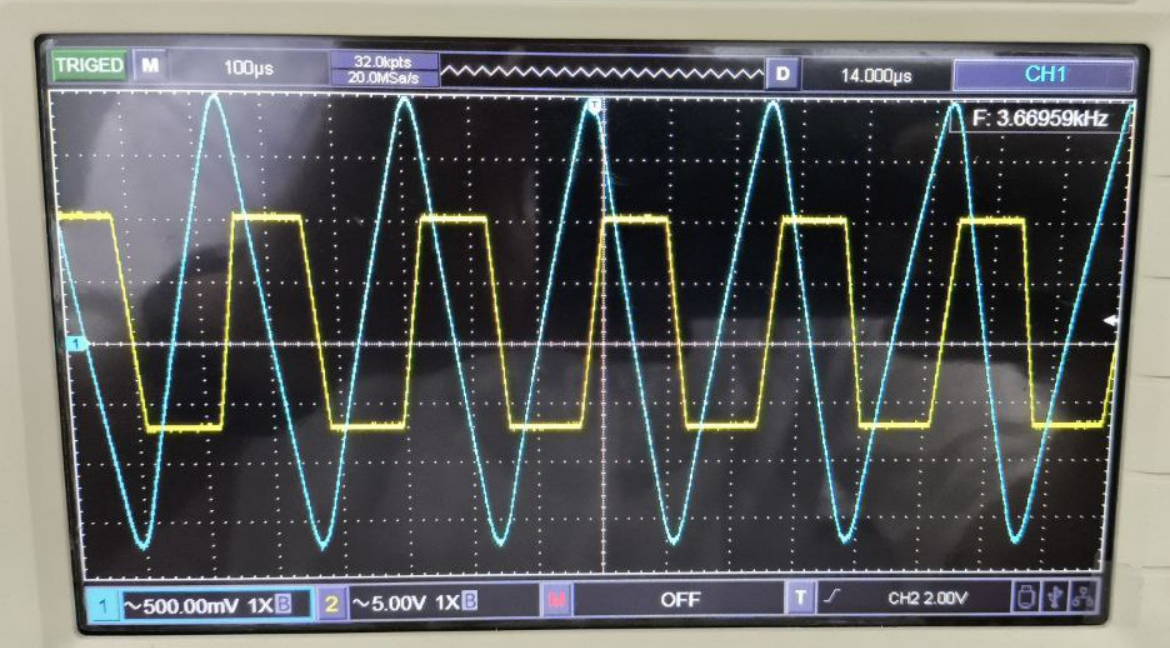
\includegraphics[width=15cm]{Imagenes/exp_gf.png}
                \caption{Señales de salida de la figura \ref{fig:gf}. Vout=Vsat:(Amarillo). Va:(Azul)}
                \label{fig:exp_gf}
            \end{figure}

            \begin{table}[H]
                \centering
                \begin{tabular}{|c|c|c|c|}
                    \hline
                    \textbf{time/div} $[s]$ & \textbf{Channel} & \textbf{voltios/div $[\volt]$} & \textbf{Acoplamiento} \\ \hline
                    $(100 \, \pm 20) \, \mu  $ & 1 (Azul)  &   $(500 \pm 100) \, m   $ & AC \\ \hline  
                    $(100 \, \pm 20 )\, \mu  $ & 2 (Amarillo)  &   $5 \pm 1   $ & AC \\ \hline  
                \end{tabular}
                \caption{Escalas Usada en el Osciloscopio Digital UNI-T UTD2102CEX+}
                \label{tab:escala_gf}
            \end{table}


             
            \begin{figure}[H]
                \centering
                \renewcommand{\figurename}{Imagen}
                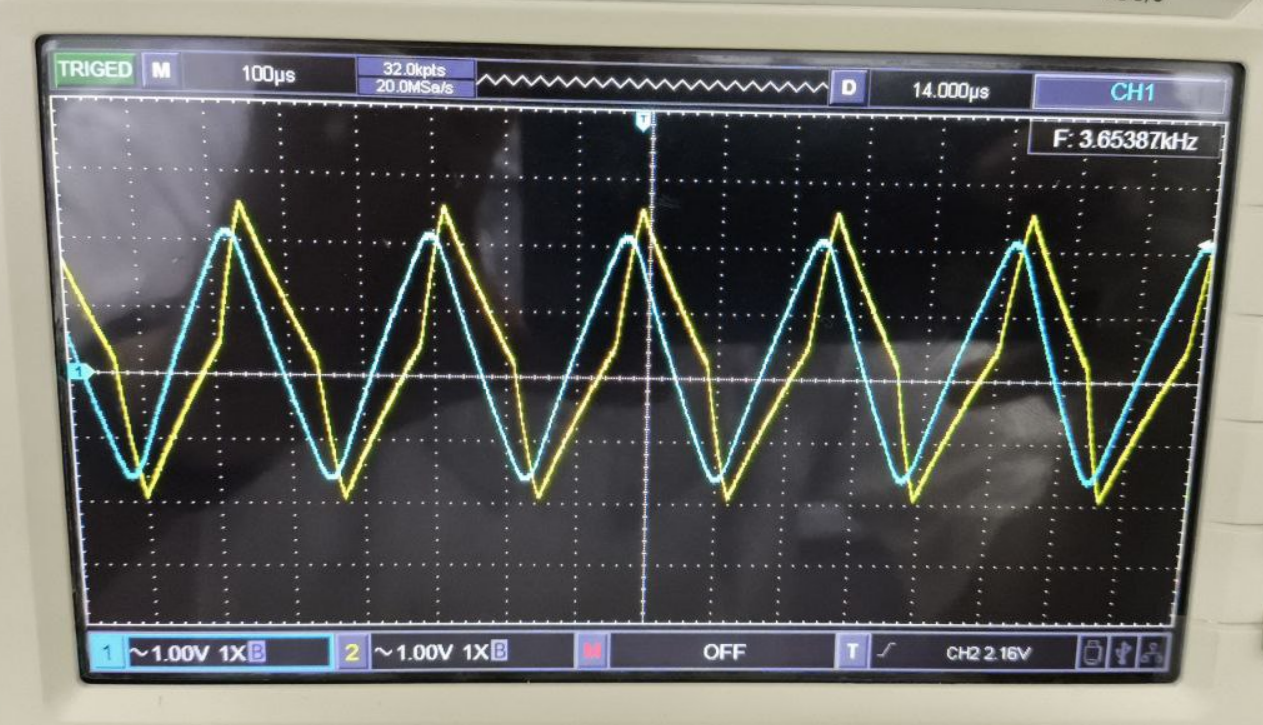
\includegraphics[width=15cm]{Imagenes/exp_gf2.png}
                \caption{Señales de salida de la figura \ref{fig:gf}. V+:(Amarillo). Va:(Azul)}
                \label{fig:exp_gf2}
            \end{figure}

            \begin{table}[H]
                \centering
                \begin{tabular}{|c|c|c|c|}
                    \hline
                    \textbf{time/div} $[s]$ & \textbf{Channel} & \textbf{voltios/div $[\volt]$} & \textbf{Acoplamiento} \\ \hline
                    $(100 \, \pm 20) \, \mu  $ & 1 (Azul)  &   $1 \pm 0.2   $ & AC \\ \hline  
                    $(100 \, \pm 20) \, \mu  $ & 2 (Amarillo)  &   $1 \pm 0.2   $ & AC \\ \hline  
                \end{tabular}
                \caption{Escalas Usada en el Osciloscopio Digital UNI-T UTD2102CEX+}
                \label{tab:escala_gf2}
            \end{table}
        


      

    
\newpage
